\begin{frame}
  \frametitle{Soft Tissue Models:  Parameter Identification}
  \begin{itemize}
  \item complex soft tissue models
    \begin{itemize}
    \item smooth, skeletal, or cardiac muscles
    \item large deformations
    \end{itemize}
  \item mixture of the extracellular \emph{matrix} and muscle \emph{fibres}
  \item \emph{automatic identification algorithm}
    \begin{itemize}
    \item many constitutive parameters to identify from \emph{measurements}
    \end{itemize}
  \end{itemize}
  \begin{center}
    \begin{minipage}{0.35\linewidth}
      \scriptsize
      quantitative microscopy \\
      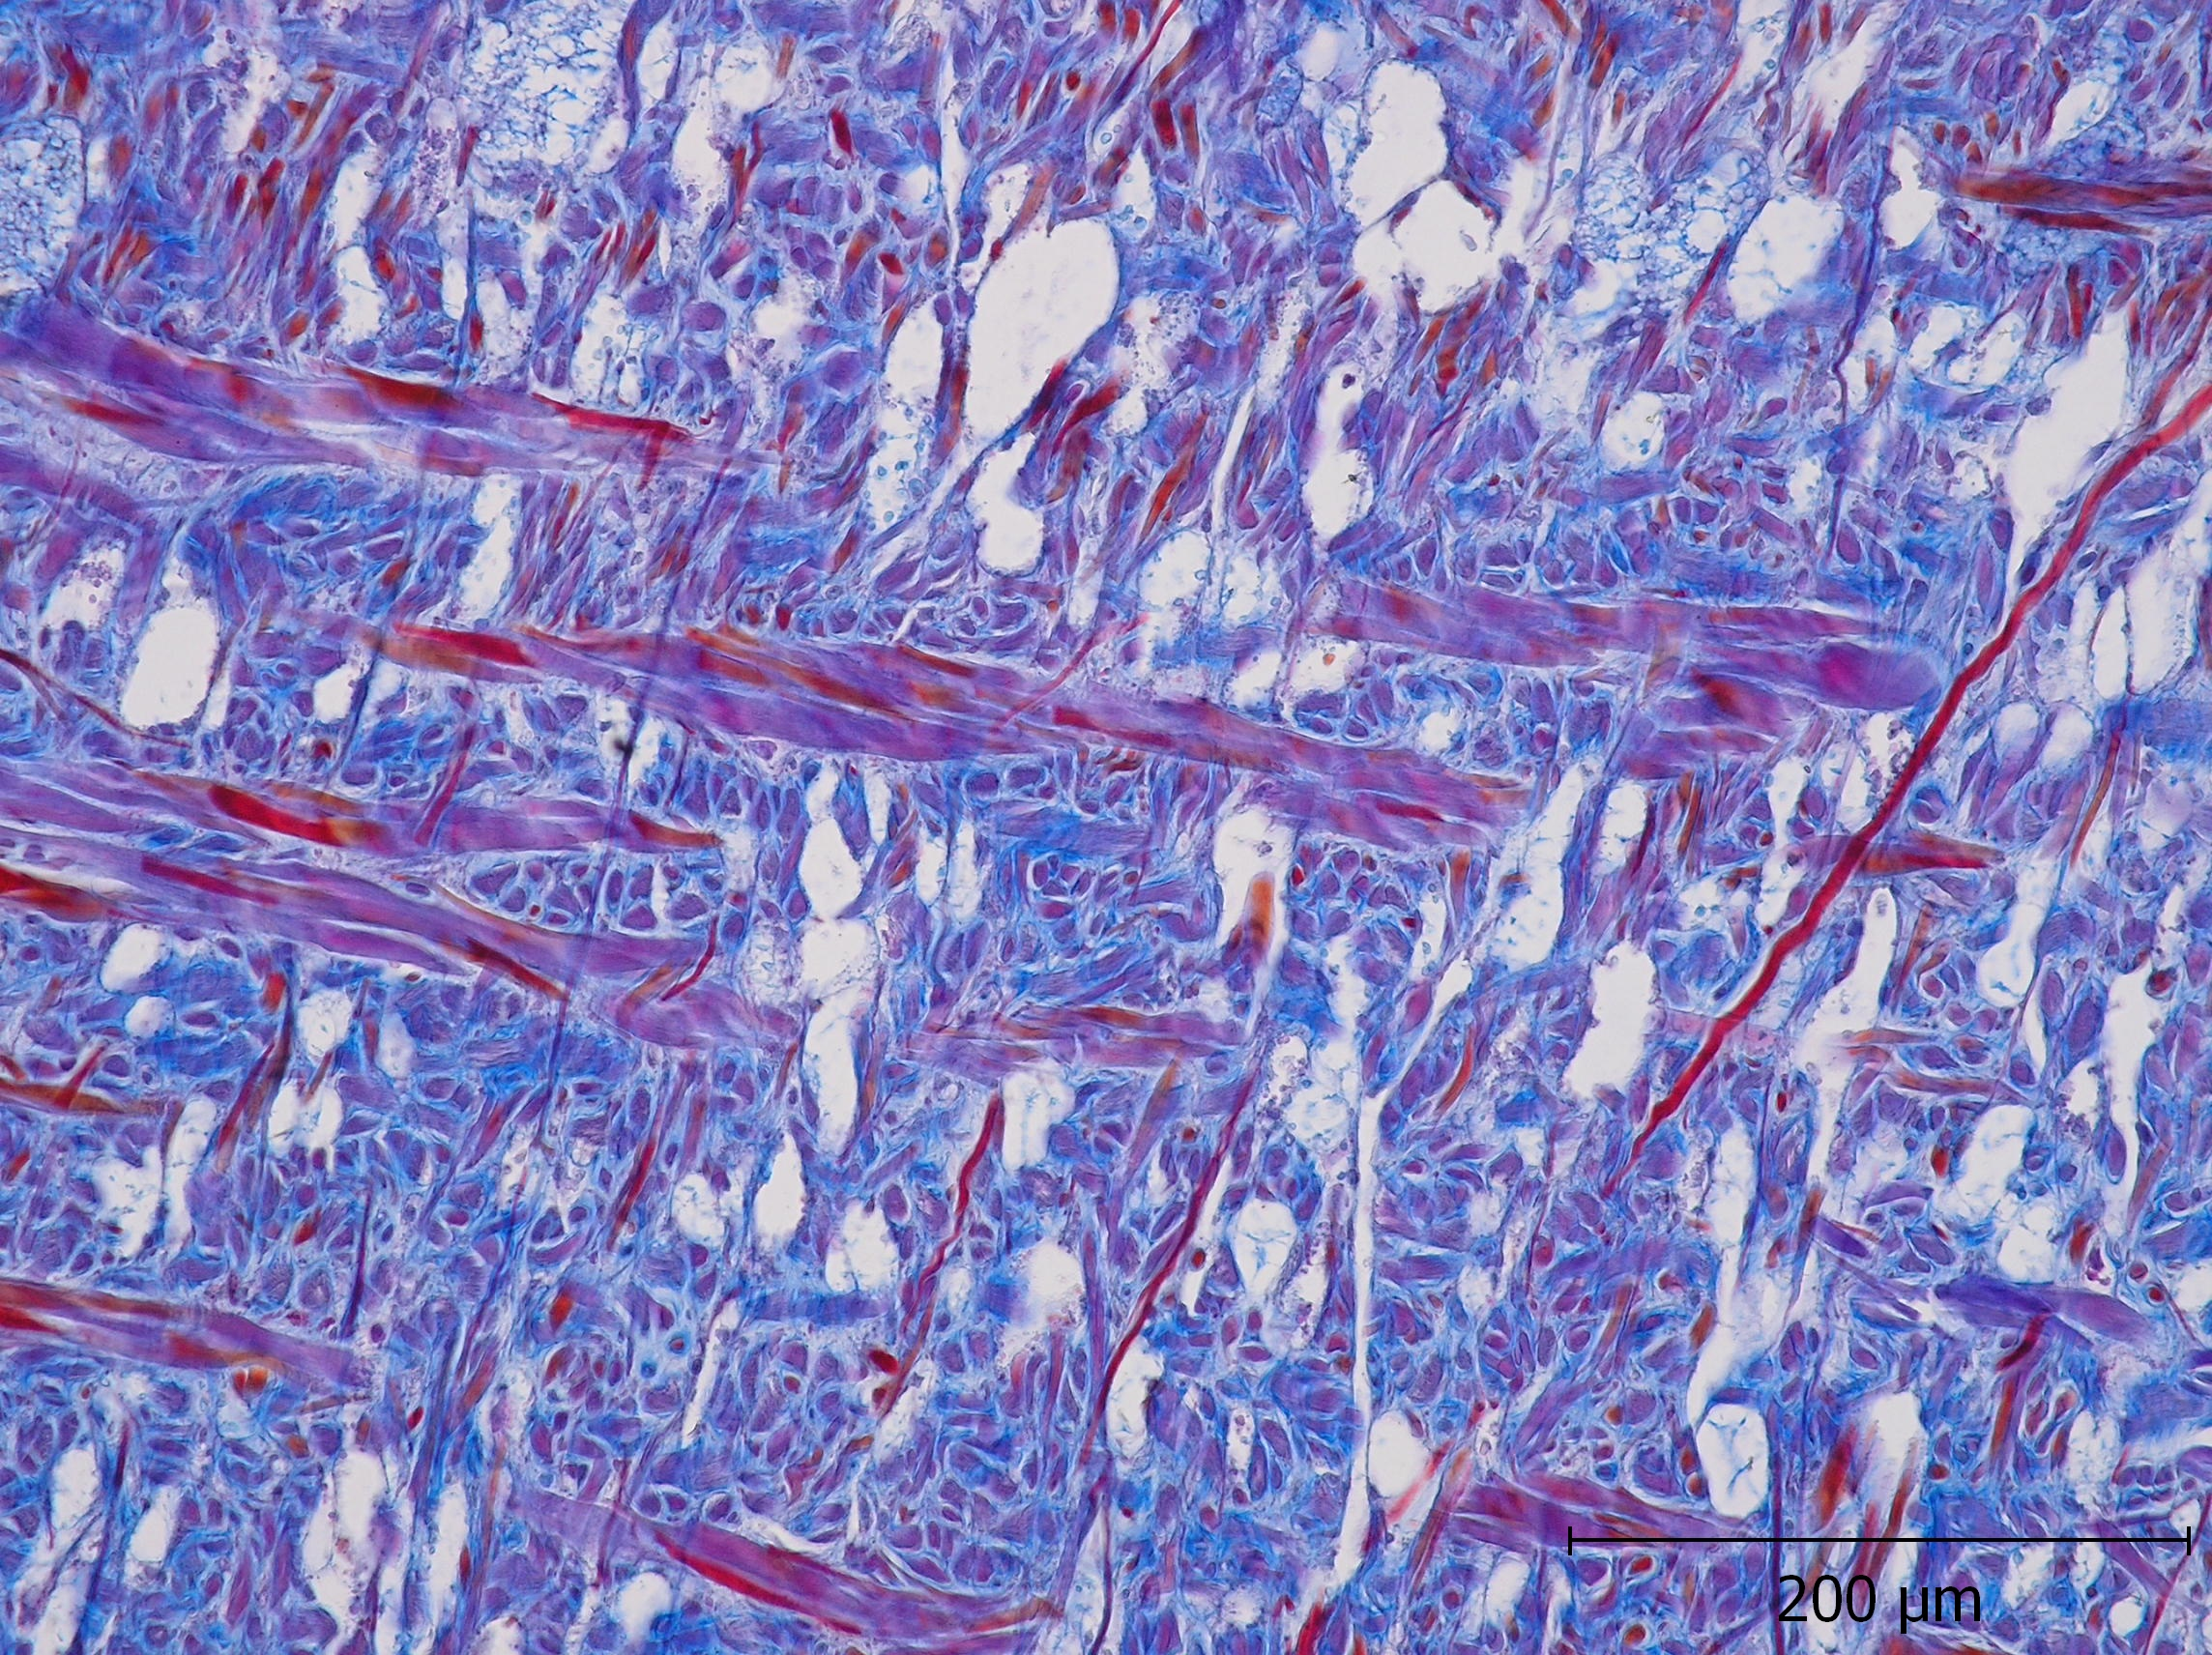
\includegraphics[width=\linewidth]{\figDirMacroIdent/51_04_02a}
    \end{minipage}
    \hfill
    \begin{minipage}{0.28\linewidth}
      \scriptsize
      finite element modeling \\
      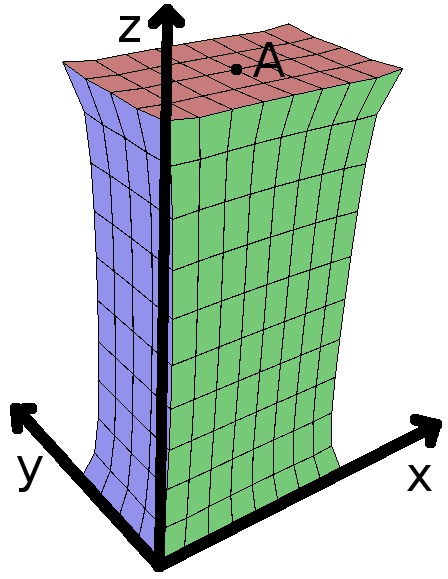
\includegraphics[width=0.8\linewidth]{\figDirMacroIdent/finaldef}
    \end{minipage}
    \hfill
    \begin{minipage}{0.35\linewidth}
      \scriptsize
      fit to measured data \\
      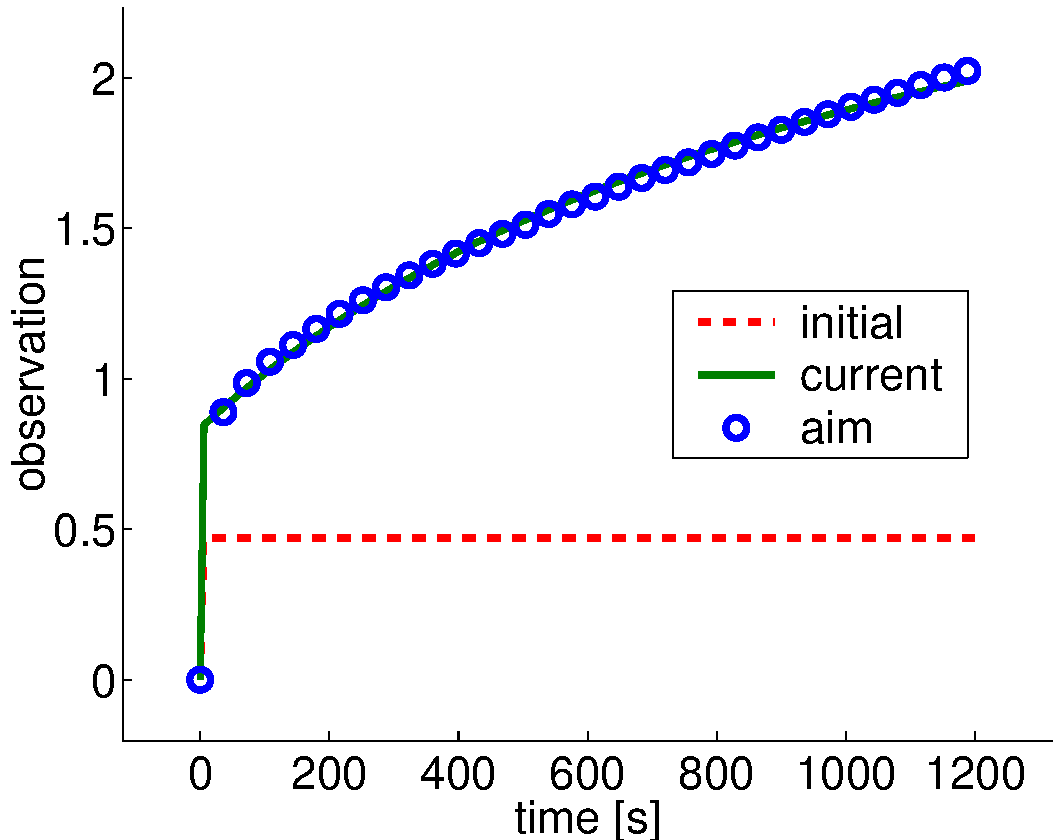
\includegraphics[width=\linewidth]{\figDirMacroIdent/saConv0022}
    \end{minipage}
  \end{center}
\end{frame}
